\documentclass{standalone}
\usepackage{tikz}
\usetikzlibrary{patterns, positioning}


\begin{document}
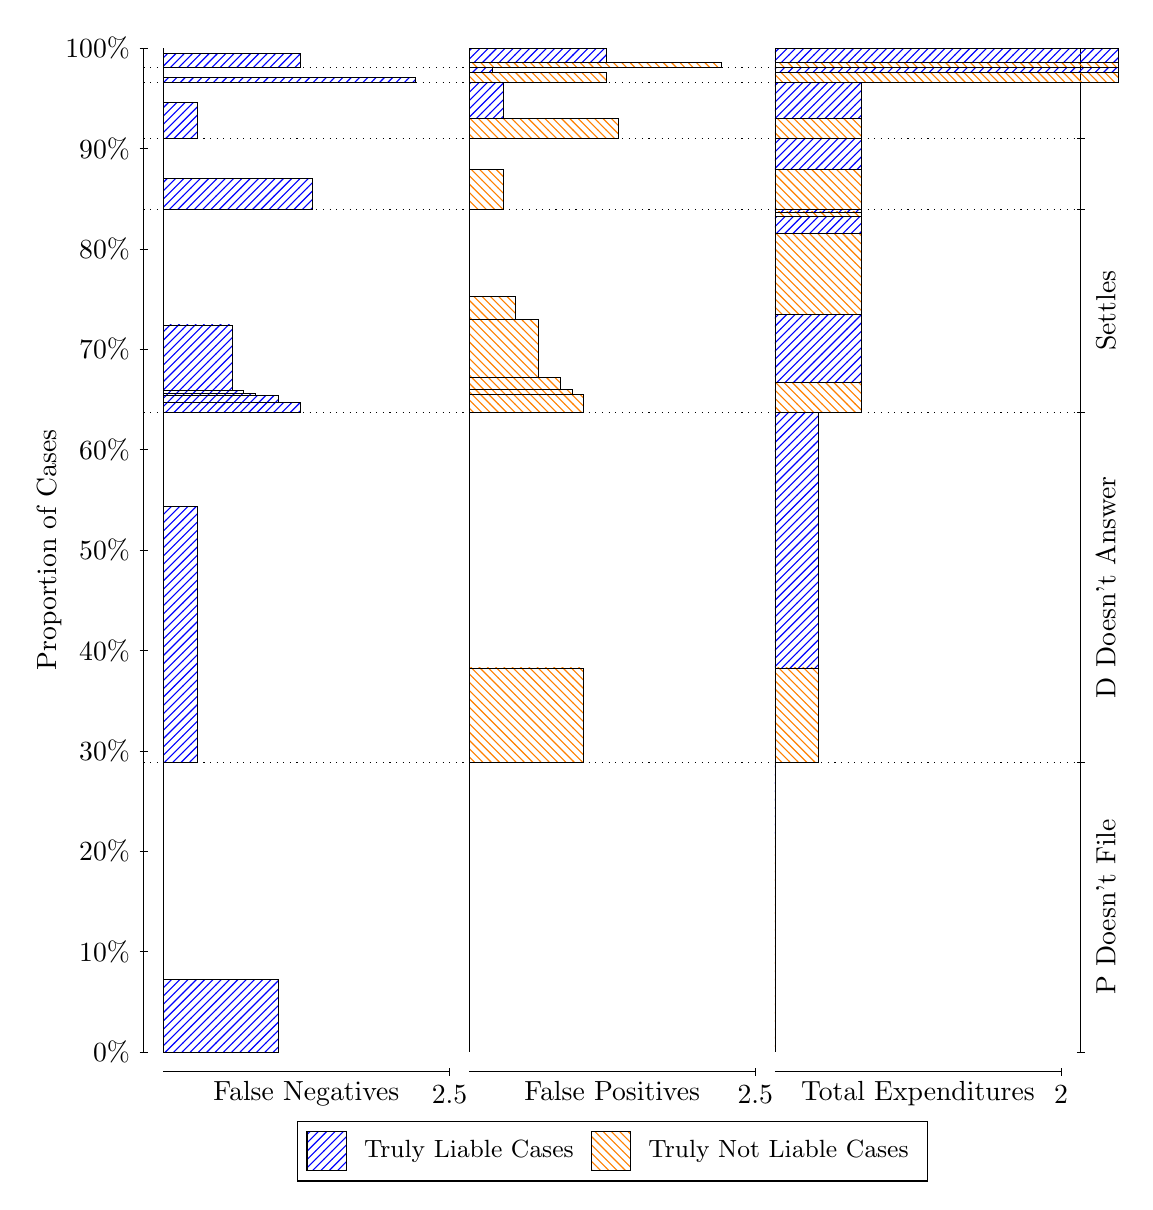
\begin{tikzpicture}
\draw[black, very thin] (1.5,1.75) -- (1.5,14.5);
\node[rotate=90, text=black, anchor=center] at (0.3, 8.125) {Proportion of Cases};
\draw[black, very thin] (1.45,1.75) -- (1.55,1.75);
\node[text=black, anchor=east] at (1.45, 1.75) {0\%};
\draw[black, very thin] (1.45,3.025) -- (1.55,3.025);
\node[text=black, anchor=east] at (1.45, 3.025) {10\%};
\draw[black, very thin] (1.45,4.3) -- (1.55,4.3);
\node[text=black, anchor=east] at (1.45, 4.3) {20\%};
\draw[black, very thin] (1.45,5.575) -- (1.55,5.575);
\node[text=black, anchor=east] at (1.45, 5.575) {30\%};
\draw[black, very thin] (1.45,6.85) -- (1.55,6.85);
\node[text=black, anchor=east] at (1.45, 6.85) {40\%};
\draw[black, very thin] (1.45,8.125) -- (1.55,8.125);
\node[text=black, anchor=east] at (1.45, 8.125) {50\%};
\draw[black, very thin] (1.45,9.4) -- (1.55,9.4);
\node[text=black, anchor=east] at (1.45, 9.4) {60\%};
\draw[black, very thin] (1.45,10.675) -- (1.55,10.675);
\node[text=black, anchor=east] at (1.45, 10.675) {70\%};
\draw[black, very thin] (1.45,11.95) -- (1.55,11.95);
\node[text=black, anchor=east] at (1.45, 11.95) {80\%};
\draw[black, very thin] (1.45,13.225) -- (1.55,13.225);
\node[text=black, anchor=east] at (1.45, 13.225) {90\%};
\draw[black, very thin] (1.45,14.5) -- (1.55,14.5);
\node[text=black, anchor=east] at (1.45, 14.5) {100\%};

\draw[black, very thin] (13.4,1.75) -- (13.4,14.5);
\draw[black, very thin] (13.35,1.75) -- (13.45,1.75);
\node[anchor=west] at (13.35, 1.75) {};
\draw[black, very thin] (13.35,5.4305) -- (13.45,5.4305);
\node[anchor=west] at (13.35, 5.4305) {};
\draw[black, very thin] (13.35,9.8755) -- (13.45,9.8755);
\node[anchor=west] at (13.35, 9.8755) {};
\draw[black, very thin] (13.35,12.452) -- (13.45,12.452);
\node[anchor=west] at (13.35, 12.452) {};
\draw[black, very thin] (13.35,13.352) -- (13.45,13.352);
\node[anchor=west] at (13.35, 13.352) {};
\draw[black, very thin] (13.35,14.064) -- (13.45,14.064);
\node[anchor=west] at (13.35, 14.064) {};
\draw[black, very thin] (13.35,14.256) -- (13.45,14.256);
\node[anchor=west] at (13.35, 14.256) {};
\draw[black, very thin] (13.35,14.5) -- (13.45,14.5);
\node[anchor=west] at (13.35, 14.5) {};

\draw[black, very thin, pattern color=blue, pattern=north east lines] (1.75,1.75) rectangle (3.2033,2.6744);
\draw[black, very thin, pattern color=orange, pattern=north west lines] (1.75,2.6744) rectangle (1.75,5.4305);
\draw[black, very thin, pattern color=blue, pattern=north east lines] (1.75,5.4305) rectangle (2.186,8.679);
\draw[black, very thin, pattern color=orange, pattern=north west lines] (1.75,8.679) rectangle (1.75,9.8755);
\draw[black, very thin, pattern color=blue, pattern=north east lines] (1.75,9.8755) rectangle (3.494,9.9948);
\draw[black, very thin, pattern color=blue, pattern=north east lines] (1.75,9.9948) rectangle (3.2033,10.089);
\draw[black, very thin, pattern color=blue, pattern=north east lines] (1.75,10.089) rectangle (2.9127,10.118);
\draw[black, very thin, pattern color=blue, pattern=north east lines] (1.75,10.118) rectangle (2.7673,10.151);
\draw[black, very thin, pattern color=blue, pattern=north east lines] (1.75,10.151) rectangle (2.622,10.984);
\draw[black, very thin, pattern color=orange, pattern=north west lines] (1.75,10.984) rectangle (1.75,12.452);
\draw[black, very thin, pattern color=blue, pattern=north east lines] (1.75,12.452) rectangle (3.6393,12.848);
\draw[black, very thin, pattern color=orange, pattern=north west lines] (1.75,12.848) rectangle (1.75,13.352);
\draw[black, very thin, pattern color=blue, pattern=north east lines] (1.75,13.352) rectangle (2.186,13.805);
\draw[black, very thin, pattern color=orange, pattern=north west lines] (1.75,13.805) rectangle (1.75,14.064);
\draw[black, very thin, pattern color=blue, pattern=north east lines] (1.75,14.064) rectangle (4.9473,14.129);
\draw[black, very thin, pattern color=orange, pattern=north west lines] (1.75,14.129) rectangle (1.75,14.256);
\draw[black, very thin, pattern color=blue, pattern=north east lines] (1.75,14.256) rectangle (3.494,14.435);
\draw[black, very thin, pattern color=orange, pattern=north west lines] (1.75,14.435) rectangle (1.75,14.5);
\draw[black, very thin, pattern color=orange, pattern=north west lines] (5.6333,1.75) rectangle (5.6333,4.5061);
\draw[black, very thin, pattern color=blue, pattern=north east lines] (5.6333,4.5061) rectangle (5.6333,5.4305);
\draw[black, very thin, pattern color=orange, pattern=north west lines] (5.6333,5.4305) rectangle (7.0867,6.627);
\draw[black, very thin, pattern color=blue, pattern=north east lines] (5.6333,6.627) rectangle (5.6333,9.8755);
\draw[black, very thin, pattern color=orange, pattern=north west lines] (5.6333,9.8755) rectangle (7.0867,10.104);
\draw[black, very thin, pattern color=orange, pattern=north west lines] (5.6333,10.104) rectangle (6.9413,10.164);
\draw[black, very thin, pattern color=orange, pattern=north west lines] (5.6333,10.164) rectangle (6.796,10.317);
\draw[black, very thin, pattern color=orange, pattern=north west lines] (5.6333,10.317) rectangle (6.5053,11.058);
\draw[black, very thin, pattern color=orange, pattern=north west lines] (5.6333,11.058) rectangle (6.2147,11.344);
\draw[black, very thin, pattern color=blue, pattern=north east lines] (5.6333,11.344) rectangle (5.6333,12.452);
\draw[black, very thin, pattern color=orange, pattern=north west lines] (5.6333,12.452) rectangle (6.0693,12.956);
\draw[black, very thin, pattern color=blue, pattern=north east lines] (5.6333,12.956) rectangle (5.6333,13.352);
\draw[black, very thin, pattern color=orange, pattern=north west lines] (5.6333,13.352) rectangle (7.5227,13.61);
\draw[black, very thin, pattern color=blue, pattern=north east lines] (5.6333,13.61) rectangle (6.0693,14.064);
\draw[black, very thin, pattern color=orange, pattern=north west lines] (5.6333,14.064) rectangle (7.3773,14.191);
\draw[black, very thin, pattern color=blue, pattern=north east lines] (5.6333,14.191) rectangle (5.924,14.256);
\draw[black, very thin, pattern color=orange, pattern=north west lines] (5.6333,14.256) rectangle (8.8307,14.321);
\draw[black, very thin, pattern color=blue, pattern=north east lines] (5.6333,14.321) rectangle (7.3773,14.5);
\draw[black, very thin, pattern color=orange, pattern=north west lines] (9.5167,1.75) rectangle (9.5167,4.5061);
\draw[black, very thin, pattern color=blue, pattern=north east lines] (9.5167,4.5061) rectangle (9.5167,5.4305);
\draw[black, very thin, pattern color=orange, pattern=north west lines] (9.5167,5.4305) rectangle (10.062,6.627);
\draw[black, very thin, pattern color=blue, pattern=north east lines] (9.5167,6.627) rectangle (10.062,9.8755);
\draw[black, very thin, pattern color=orange, pattern=north west lines] (9.5167,9.8755) rectangle (10.607,10.258);
\draw[black, very thin, pattern color=blue, pattern=north east lines] (9.5167,10.258) rectangle (10.607,11.119);
\draw[black, very thin, pattern color=orange, pattern=north west lines] (9.5167,11.119) rectangle (10.607,12.146);
\draw[black, very thin, pattern color=blue, pattern=north east lines] (9.5167,12.146) rectangle (10.607,12.36);
\draw[black, very thin, pattern color=orange, pattern=north west lines] (9.5167,12.36) rectangle (10.607,12.419);
\draw[black, very thin, pattern color=blue, pattern=north east lines] (9.5167,12.419) rectangle (10.607,12.452);
\draw[black, very thin, pattern color=orange, pattern=north west lines] (9.5167,12.452) rectangle (10.607,12.956);
\draw[black, very thin, pattern color=blue, pattern=north east lines] (9.5167,12.956) rectangle (10.607,13.352);
\draw[black, very thin, pattern color=orange, pattern=north west lines] (9.5167,13.352) rectangle (10.607,13.61);
\draw[black, very thin, pattern color=blue, pattern=north east lines] (9.5167,13.61) rectangle (10.607,14.064);
\draw[black, very thin, pattern color=orange, pattern=north west lines] (9.5167,14.064) rectangle (13.877,14.191);
\draw[black, very thin, pattern color=blue, pattern=north east lines] (9.5167,14.191) rectangle (13.877,14.256);
\draw[black, very thin, pattern color=orange, pattern=north west lines] (9.5167,14.256) rectangle (13.877,14.321);
\draw[black, very thin, pattern color=blue, pattern=north east lines] (9.5167,14.321) rectangle (13.877,14.5);
\draw[black, dotted] (1.5,5.4305) -- (13.4,5.4305);
\draw[black, dotted] (1.5,9.8755) -- (13.4,9.8755);
\draw[black, dotted] (1.5,12.452) -- (13.4,12.452);
\draw[black, dotted] (1.5,13.352) -- (13.4,13.352);
\draw[black, dotted] (1.5,14.064) -- (13.4,14.064);
\draw[black, dotted] (1.5,14.256) -- (13.4,14.256);
\draw[black, very thin] (1.75,1.5) -- (5.3833,1.5);
\node[text=black, anchor=north] at (3.5667, 1.5) {False Negatives};
\draw[black, very thin] (5.3833,1.45) -- (5.3833,1.55);
\node[text=black, anchor=north] at (5.3833, 1.45) {2.5};

\draw[black, very thin] (5.6333,1.5) -- (9.2667,1.5);
\node[text=black, anchor=north] at (7.45, 1.5) {False Positives};
\draw[black, very thin] (9.2667,1.45) -- (9.2667,1.55);
\node[text=black, anchor=north] at (9.2667, 1.45) {2.5};

\draw[black, very thin] (9.5167,1.5) -- (13.15,1.5);
\node[text=black, anchor=north] at (11.333, 1.5) {Total Expenditures};
\draw[black, very thin] (13.15,1.45) -- (13.15,1.55);
\node[text=black, anchor=north] at (13.15, 1.45) {2};

\node[text=black, centered, rotate=90] at (13.72, 3.5902) {P Doesn't File};
\node[text=black, centered, rotate=90] at (13.72, 7.653) {D Doesn't Answer};
\node[text=black, centered, rotate=90] at (13.72, 11.164) {Settles};





\draw (7.449999999999999,1.5) node[draw=none] (baseCoordinate) {};
\begin{scope}[align=center]
        \matrix[scale=0.5, draw=black, below=0.5cm of baseCoordinate, nodes={draw}, column sep=0.1cm]{
            \node[rectangle, draw, minimum width=0.5cm, minimum height=0.5cm, pattern color=blue, pattern=north east lines] {}; &
            \node[draw=none, font=\small, text=black] (B) {Truly Liable Cases}; &
            \node[rectangle, draw, minimum width=0.5cm, minimum height=0.5cm, pattern color=orange, pattern=north west lines] {}; &
            \node[draw=none, font=\small, text=black] (B) {Truly Not Liable Cases}; \\
            };
\end{scope}

\end{tikzpicture}
\end{document}